\documentclass[12pt,a4paper]{article}

% Paquetes esenciales para artículos de Ciberseguridad
\usepackage{cite}
\usepackage{amsmath,amssymb,amsfonts}
\usepackage{algorithm}
\usepackage{algpseudocode}
\usepackage{graphicx}
\usepackage{textcomp}
\usepackage{xcolor}
\usepackage{booktabs}
\usepackage{array}
\usepackage{multirow}
\usepackage{siunitx}
\usepackage{listings}

\usepackage{tikz}
\usetikzlibrary{shapes,arrows,positioning,fit,backgrounds,calc}
\usepackage{pgfplots}

\pgfplotsset{compat=1.16}

\usepackage{hyperref}
\usepackage{tabularx}
\usepackage{enumitem}
\usepackage{mdframed}
\usepackage[left=2.5cm,right=2.5cm,top=2.5cm,bottom=2.5cm]{geometry}
\usepackage{authblk} % Para gestionar autores y afiliaciones de manera sencilla

\usepackage[spanish]{babel} % idioma en español
\usepackage{float}


% Definición de colores para ciberseguridad
\definecolor{alertred}{RGB}{235,54,42}
\definecolor{warningyellow}{RGB}{250,190,40}
\definecolor{securegreen}{RGB}{46,204,113}
\definecolor{infoblue}{RGB}{52,152,219}
\definecolor{vulnerablepurple}{RGB}{155,89,182}
\definecolor{codegray}{RGB}{240,240,240}
\definecolor{commentgreen}{RGB}{63,127,95}
\definecolor{codeblue}{RGB}{0,0,255}
\definecolor{codered}{RGB}{176,0,0}
\definecolor{cryptogreen}{RGB}{0,128,0}
\definecolor{encryptionbg}{RGB}{245,245,245}

% Configuración para listings con soporte mejorado para bash
\lstdefinelanguage{Bash}{
  keywords={if, then, else, elif, fi, for, do, done, while, until, case, esac, function},
  keywordstyle=\color{blue},
  sensitive=true,
  comment=[l]{\#},
  commentstyle=\color{commentgreen},
  stringstyle=\color{red!70!black},
  morestring=[b]",
  morestring=[b]'
}

% Definición para código fuente genérico incluyendo lenguajes de programación comunes
\lstdefinestyle{codestyle}{
    basicstyle=\ttfamily\small,
    keywordstyle=\color{codeblue},
    stringstyle=\color{codered},
    commentstyle=\color{commentgreen},
    showstringspaces=false,
    numbers=left,
    numberstyle=\tiny\color{gray},
    numbersep=5pt,
    frame=single,
    backgroundcolor=\color{codegray},
    breaklines=true,
    breakatwhitespace=true,
    tabsize=4,
    captionpos=b,
    literate=
        {\$}{{{\color{codeblue}\$}}}1
        {>}{{{\color{codered}\textgreater}}}1
        {<}{{{\color{codered}\textless}}}1
        {|}{{{\color{codered}|}}}1
        {&}{{{\color{codered}\&}}}1
}

% Definición para mostrar algoritmos criptográficos o pseudocódigo
\lstdefinestyle{cryptoalgo}{
    basicstyle=\ttfamily\small,
    keywordstyle=\color{cryptogreen}\bfseries,
    stringstyle=\color{codered},
    commentstyle=\color{commentgreen}\itshape,
    showstringspaces=false,
    numbers=left,
    numberstyle=\tiny\color{gray},
    numbersep=5pt,
    frame=single,
    backgroundcolor=\color{encryptionbg},
    breaklines=true,
    breakatwhitespace=true,
    tabsize=4,
    captionpos=b,
    emphstyle=\color{blue},
    emph={permutación, expansión, sustitución, rotación, desplazamiento, cifrado, descifrado, bloque, ronda, clave}
}

\lstset{
    breaklines=true,
    breakatwhitespace=true,
    style=codestyle,
    frame=single,
    showstringspaces=false,
    columns=flexible
}

% Estilos para bloques de alerta de seguridad
\newmdenv[
  linecolor=alertred,
  backgroundcolor=alertred!10,
  frametitle={Alerta de Seguridad},
  frametitlebackgroundcolor=alertred!40,
  frametitlefont=\bfseries\color{white},
  roundcorner=4pt
]{securityalert}

\newmdenv[
  linecolor=warningyellow,
  backgroundcolor=warningyellow!10,
  frametitle={Advertencia},
  frametitlebackgroundcolor=warningyellow!40,
  frametitlefont=\bfseries\color{black},
  roundcorner=4pt
]{securitywarning}

\newmdenv[
  linecolor=securegreen,
  backgroundcolor=securegreen!10,
  frametitle={Buena Práctica},
  frametitlebackgroundcolor=securegreen!40,
  frametitlefont=\bfseries\color{white},
  roundcorner=4pt
]{securitygoodpractice}

% Definición para métodos criptográficos
\newmdenv[
  linecolor=infoblue,
  backgroundcolor=infoblue!5,
  frametitle={Método Criptográfico},
  frametitlebackgroundcolor=infoblue!40,
  frametitlefont=\bfseries\color{white},
  roundcorner=4pt
]{cryptomethod}

% Definición para análisis criptográfico
\newmdenv[
  linecolor=vulnerablepurple,
  backgroundcolor=vulnerablepurple!5,
  frametitle={Análisis Criptográfico},
  frametitlebackgroundcolor=vulnerablepurple!40,
  frametitlefont=\bfseries\color{white},
  roundcorner=4pt
]{cryptoanalysis}

% Definición de BibTeX
\def\BibTeX{{\rm B\kern-.05em{\sc i\kern-.025em b}\kern-.08em
    T\kern-.1667em\lower.7ex\hbox{E}\kern-.125emX}}

\begin{document}

\title{\LARGE \textbf{Laboratorio: Protocolos Seguros y Seguridad Perimetral}}

\author{\textbf{Profesor Gustavo Adolfo Echeverri\\}}
\author[1]{Juan Carlos Charfuelan Caipe}
\author[2]{Fabian Alberto Guancha Vera}
\author[3]{Over Haider Castrillón Valencia}

\affil[1]{Departamento de Ingeniería en Sistemas y Computación, Universidad de Caldas}
\affil{Manizales, Colombia}
\date{\today}
\maketitle

\section*{Introducción}
Este laboratorio presenta la implementación de una suite completa de cifrado utilizando las
bibliotecas criptográficas de Python. Se abordan conceptos fundamentales de la criptografía moderna
incluyendo funciones hash, firmas digitales, cifrado simétrico y asimétrico, y criptografía de
curvas elípticas. Cada implementación se acompaña de explicaciones teóricas, código funcional y
análisis de seguridad.

\section{Configurar y Desplegar un Web Server Seguro TLS/SSL}

\subsection{Implementación mediante OpenSSL + Python}

\subsubsection{Generación de Certificados SSL/TLS}

Se generó un certificado autofirmado utilizando OpenSSL para establecer una
conexión segura HTTPS con el servidor web desarrollado en Python.

\begin{lstlisting}[language=bash, caption=Comando para generar certificado autofirmado]
openssl req -nodes -x509 -newkey rsa:4096 -keyout key.pem -out cert.pem -days 365 -subj '/CN=localhost/O=UCM'
\end{lstlisting}

\textbf{Parámetros del comando explicados:}

\begin{itemize}
  \item \textbf{\texttt{-nodes}}: No cifra la clave privada con contraseña, permitiendo que el servicio se reinicie automáticamente sin intervención manual
  \item \textbf{\texttt{-x509}}: Genera un certificado autofirmado en formato X.509
  \item \textbf{\texttt{-newkey rsa:4096}}: Crea una nueva clave RSA de 4096 bits para mayor seguridad
  \item \textbf{\texttt{-keyout key.pem}}: Especifica el archivo donde se guardará la clave privada
  \item \textbf{\texttt{-out cert.pem}}: Define el archivo de salida para el certificado público
  \item \textbf{\texttt{-days 365}}: Establece la validez del certificado por 365 días
  \item \textbf{\texttt{-subj '/CN=localhost/O=UCM'}}: Define el nombre común (localhost) y la organización (UCM)
\end{itemize}

\begin{figure}[H]
  \centering
  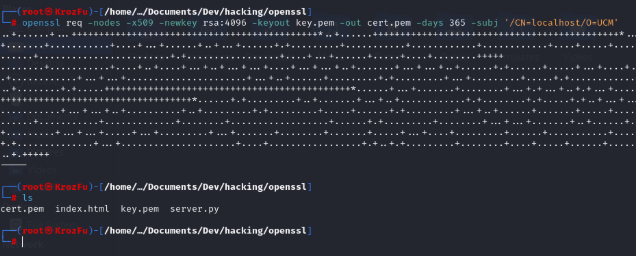
\includegraphics[width=0.75\textwidth]{./assets/img1.png}
  \caption{Proceso de generación del certificado SSL/TLS}
  \label{fig:cert-generation}
\end{figure}

\subsubsection{Archivos de Certificado Generados}

\textbf{Clave Privada (key.pem)}

El archivo \texttt{key.pem} contiene la clave privada RSA de 4096 bits
utilizada para el cifrado:

\begin{lstlisting}[caption=Private Key]
--BEGIN PRIVATE KEY-----
MIIJQgIBADANBgkqhkiG9w0BAQEFAASCCSWwggkoAgEAAoICAQDV6Z8V4Qrgh1I0
Km+RrlYvPoQspwAMp016ZudRyzrad3511khTo/f4GWxgBJhfgCa/NUCvxDchCpG3
NRNGLSYTfiLiYNiNpLZL02YdbxopdbBI5nvkTyiAFMus@DQ5UhH8D4M4TXoWlWo
MISammeQ2W5PnwvHtNYmc6F+9180YJ8hdukY7TL9Vs0J4vYVXaoudC4mAJmS7kon
hsXw5jcCk19e9thy/rjDsigiMZqI/4Wjr44aW9rYu+/aWEMbeRywYQJG4f8slIQX
aYRpTTLF9F9E8BH302NSBjVW2otalsynkvaplX150FLr789AIH/HEj7bi5aCFgTO
8RVgmgDØVA+jBvKLaALvm2YDxwtwu+2WwezQW19/7nFxGxRdrXVL3AXMBEMгPXP
TyH9KdEkAhbSQxuqq+1Uenm+775nFbh7mG8t0th1RvQg6R06QYdHfiws140zy Ks
UMDMHFw7XW4hEWxx8RyBPlaxADNHAihvkn5C95QSYTIt650RPbjdogRKbFMNGkJ5
HIRjkCzE/UxmjZ2atuUTo0+igIaRRsh0050EDC/LMj07mHTwJm0tv0dmc9A/XSK
nribcaWOH42y3KPiDv99Flikkk8i+j6qPqzTaq1511HRKNY07U4XusfxFQRgk3pM
dbwyc6cKON+QRBTF5C2nEFoxMvB/gQIDAQABAoICAAn9YOZQKpZeq2eVPb2TYyHØ
r0565AUzJFYbfRzOPSzbnLGhFCKXyyoyYb3AKS94iBawXMD2kE4QaLJHzvNTmG1
p8M8sr6A5u2uiFSg1uoaKIO/e15WLXsxQbEyHMpEktINNZCbac20fmaK0X54zHJW
VRCJ0F6EouwLy9RmblHREE1bRGY40wNCrIIBb9WCmME4xbjvmTxj1wGwKQk9bv83
S6JFK69/FrjI1pf2Mg3IxQBmX9/6PyeU6zgKnCOpzb2s4hLWVfjKfLqtKkpSmRbm
eRZ6kZQ9smsvsAj8zroo6156LGex+/iUlJrBCbAodF8jCn1tMNulVJcnagSnXHj2
oqSZwo7TKrzy8UyL4dqd2xPPsou76zt/RcGWPgJ12Tpv2BHE4UTxeGw/9ySbP8nc
UpXdxJqu1fMggTNsTxq7YTpqO1J4W010Lp8ruNNUDUlXiIsJcjZ9yiT+4vkez7f7
q86T9C9TueOARPWU1b5y4DNJ1n06807MOdaGqY8Q7/zN7506+PMQ1ME3L6i5e7vk
sE5mfnGjW7JthxN1nMm6ZbkQTQPHfXbwfqzbUiA40/oe0QG10tabØR10MoxfLXEO
1qTgHRNLybmVcwdhG63Vhj4t/H6FyY/hZKfm/w5cGvYEAqdJLsLhteEoMR6ky8U0
gQtU/Y1HT9tISEDfMGCZAoIBAQDqSEa7fyZVAxR2FSSGztgj2lWWZmZ1q+d8zqcG
tzd2VWeCCcfdkAymZ8pN5Yp1eNyHu/7iQeSxf9610eZm8x31tlxv@AyPmQaWsbZP
8RY7sNtPPshldp/x0T2uFK6KDHXHKAxx+3NQ7ew3GBWvag8Q0hvXSZtguhbwB+Tt
sJXt+oIpB4ZrbH1YmHG+zLSZShddEUmwDL4k2ykhkD6yfwccu7t0MF3TSCMha@Ry
9v3vgT14b5V1vPZfBoxWShTuXqKpHVAsXpGiJ2rd1KuHlmFpzsYU6KeJydFGTREU
12v10rjXHa43K1s5q2JD93V02/ZgSeZrIF3+ua3hh0VxnZwVAoIBAQDpv7qdSOSU
hQiKXRg3131AeTznEAMVzVqbj9ntffyAbd9QrV1dwTmHHN4JgZZeMRE6MIISJTh
+eD3NnS+SKBunvnbS/gpYRuQmvfulJrU+nusR/KNZ+3Pmm/YgF6SJLYJuTL29Ja+
hw+kCoHm8v9EilBnM9VXVqPPIXB5DIjs3nUTW8Zf/d6eFnOcC28L8FKqtjufTdmI
ryK9gz/HgoYn9WGaCirRXFcfg/zr1vHXmk7rXEw44ICKW1FGohZzELJ52gNaE8Ld
bi97gcVA1gmGZJ+t6cUNrMV411fA//y5/5sI1LKMX0Shu011f2JHCUVikJqbutx
/txFXMouYDS9AoIBAQCYZ6YjyKYd/V/tJPna/GncgObwbQzFrRtstF4xXzSkNRCd
plEvT8r64V/YZq841gQYBHLdqvHjigRN8eEZLaRQT944GoZhT7HajAbGYFYPRJCW
L4hbgNyxiWVvfiLAYTRA9uJROMQrYXRnUhWEU91RefgmBCMzuGnCeuhuBMAecr8
d9m4vhr+SEUOUspVQb6LG3jtHoz/GtbZ76TppvrwdSuPfPs805wm3 Ent48DzcgaT
9zqfsVowH01kJNMS8dss21XSVz6z1qKNZhCjpm7+TrXK2kJKv0/1RKdHew/EtNzr
i3J0j1TL4jKNdkghWgofP102cpr53uU/ZJ2B2H61A0IBACTbpLN0cQay53x13YG2
kbVdaksOrU3dFxcHN1xFJ0WaT7KiuDZDhDQ8vEBvzoSBNIGhKidwoKlZW43fulze
2t1WmBNqUUFFHLGangmyyQ9YR/QMjUr931PkCErdQwxMWaAC4FRq8PIuHdtCBOXD
31iRbsg3NibFdKMOpMuRnG2Tky1Jfyw7U+EPsqWSvZY+NAOWCxwfCK/avzzGzV8
cwcPnEpL3CCTLPG9NicCB7R1koguT56QWPrbF1/J4zxVn67zH6AuiYWdAE07XLøy
guH8L+meeQIFAkZXNWjLdLBni6y4tcbIpuvRWykbCS17kKVq3bombcD8YQNW9FKH
vQkCggEAbS1Bx5k92UsAaixGGAKzgERTdhE5NzZrQ/faFmOmYYBNPKZSu4JsyfAG
@kk1+uwU8em0uUcrLTZDOmNnTRakkruxek7PJd/mAcGu41T5UN/ve9DfcQj7MRx9
z2VhM/RB3z/Zyoskzq4/CIikPRrA@ImDRtenEdQaMDN1/cKLktd4oJuAmOCYBGnA
mfMcF7US1hsGFgX0n5RikPNbfAdSoNKkrdneohuXFPXQ06TAvQj+rU/MCiD+b
zhm09n6gfAUTLAHRRyvqtcRiY7DKVqcQ7ZhXGxnZJL1TndKhj/40/58hTQysheNS
KPqQ3LsmoHLeqeSCaV/f5hPPP Na2g==
-----END PRIVATE KEY-----
\end{lstlisting}

\textbf{Certificado Público (cert.pem)}

\begin{figure}[H]
  \centering
  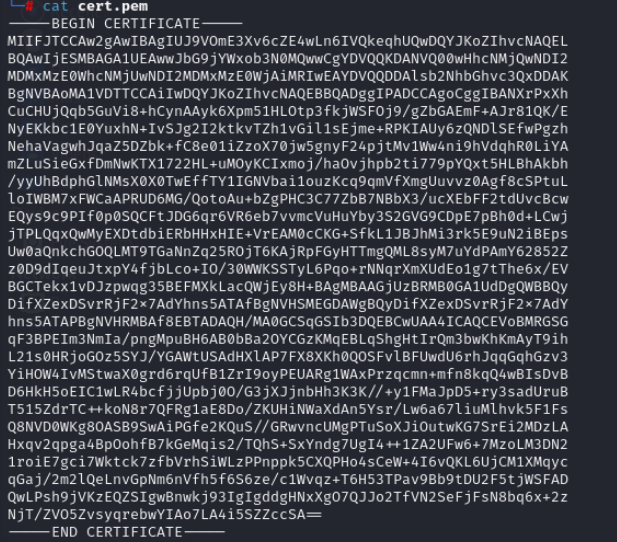
\includegraphics[width=0.75\textwidth]{./assets/img2.png}
  \caption{Contenido del certificado público X.509}
  \label{fig:cert-content}
\end{figure}

\subsubsection{Desarrollo de la Página Web de Prueba}

Se creó una página HTML simple para demostrar el funcionamiento del servidor
HTTPS:

\begin{lstlisting}[language=html, caption=Página web de prueba para el servidor HTTPS]
<!DOCTYPE html>
<html lang="es">
<head>
    <meta charset="UTF-8" />
    <meta name="viewport" content="width=device-width, initial-scale=1.0" />
    <title>Servidor Seguro UCM</title>
</head>
<body>
    <h1>Página Segura con SSL/TLS</h1>
    <p>
        Esta página web está protegida por un certificado SSL/TLS autofirmado 
        generado con OpenSSL. La comunicación entre el cliente y el servidor 
        está cifrada utilizando protocolos TLS.
    </p>
</body>
</html>
\end{lstlisting}

\subsubsection{Implementación del Servidor HTTPS en Python}

El servidor web se implementó utilizando las librerías estándar de Python,
incorporando soporte SSL/TLS:

\begin{lstlisting}[language=python, caption=Servidor HTTPS con certificados SSL/TLS]
from http.server import HTTPServer, SimpleHTTPRequestHandler
import ssl
import os

# Configuración del servidor
port = 9001
httpd = HTTPServer(('0.0.0.0', port), SimpleHTTPRequestHandler)

# Configuración de los certificados SSL/TLS
httpd.socket = ssl.wrap_socket(httpd.socket,
                              keyfile='key.pem',
                              certfile='cert.pem',
                              server_side=True)

print(f"Servidor HTTPS ejecutándose en https://0.0.0.0:{port}")
httpd.serve_forever()
\end{lstlisting}

\textbf{Componentes del servidor:}

\begin{itemize}
  \item \textbf{HTTPServer}: Servidor HTTP básico de Python
  \item \textbf{SimpleHTTPRequestHandler}: Manejador para servir archivos estáticos
  \item \textbf{ssl.wrap\_socket()}: Envuelve el socket con capacidades SSL/TLS
  \item \textbf{Puerto 9001}: Puerto personalizado para evitar conflictos con servicios estándar
\end{itemize}

\subsection{Pruebas de Funcionamiento y Verificación}

\subsubsection{Acceso al Servidor HTTPS}

Al acceder al servidor mediante un navegador web, se observa el comportamiento
típico de un certificado autofirmado:

\begin{figure}[H]
  \centering
  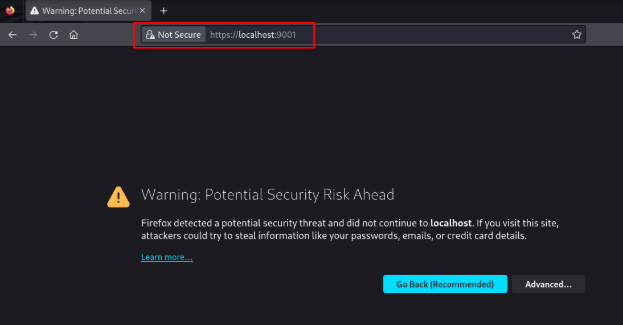
\includegraphics[width=0.75\textwidth]{./assets/img3.png}
  \caption{Advertencia de seguridad del navegador por certificado autofirmado}
  \label{fig:browser-warning}
\end{figure}

\begin{figure}[H]
  \centering
  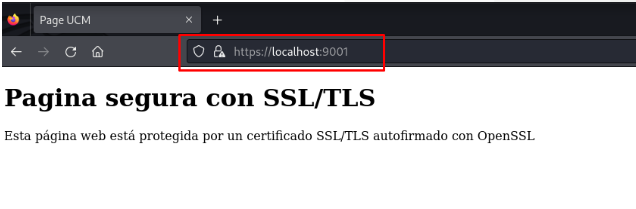
\includegraphics[width=0.75\textwidth]{./assets/img4.png}
  \caption{Página web cargada exitosamente a través de HTTPS}
  \label{fig:secure-page}
\end{figure}

\subsubsection{Verificación de Certificados}

El navegador permite inspeccionar los detalles del certificado SSL/TLS:

\begin{figure}[H]
  \centering
  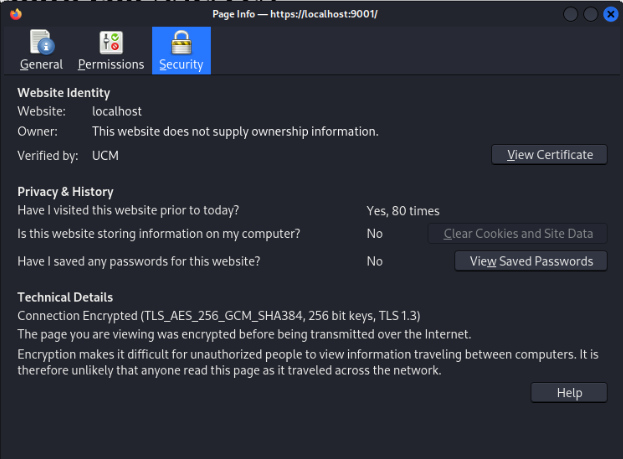
\includegraphics[width=0.75\textwidth]{./assets/img5.png}
  \caption{Información detallada del certificado SSL/TLS}
  \label{fig:cert-details}
\end{figure}

\begin{figure}[H]
  \centering
  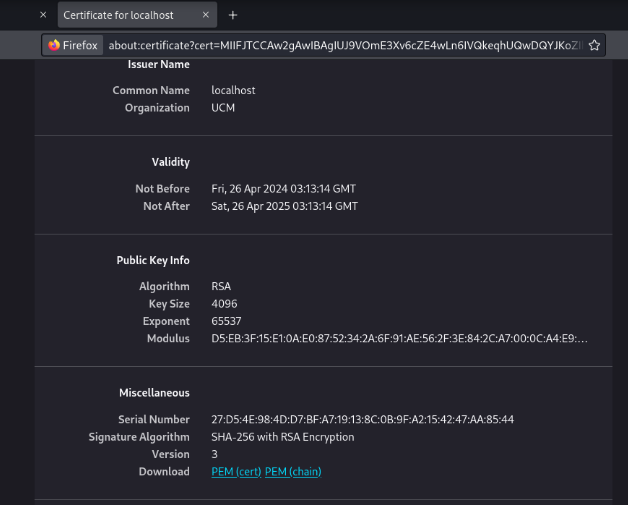
\includegraphics[width=0.75\textwidth]{./assets/img6.png}
  \caption{Verificación de la cadena de certificados y algoritmos de cifrado}
  \label{fig:cert-chain}
\end{figure}

% ----------------------------------------------------------------
\section{Firma y Verificación de Documentos con PGP}

\subsection{Implementación de Firma Digital}

\subsubsection{Generación de Clave PGP}

Para iniciar el proceso de firma digital, primero generamos un par de claves
PGP utilizando GnuPG. Ejecutamos el comando de generación completa de claves:

\begin{lstlisting}[language=bash, caption=Generación de clave PGP con GnuPG]
gpg --full-generate-key
\end{lstlisting}

El sistema presenta las siguientes opciones de algoritmos criptográficos.
Seleccionamos la opción 4 (RSA sign only) para crear una clave específicamente
para firma digital:

\begin{lstlisting}[language=text, caption=Proceso interactivo de generación de clave PGP, breaklines=true]
gpg (GnuPG) 2.4.7; Copyright (C) 2024 g10 Code GmbH
This is free software: you are free to change and redistribute it.
There is NO WARRANTY, to the extent permitted by law.

gpg: keybox '/home/krozfu/.gnupg/pubring.kbx' created
Please select what kind of key you want:
   (1) RSA and RSA
   (2) DSA and Elgamal
   (3) DSA (sign only)
   (4) RSA (sign only)
   (9) ECC (sign and encrypt) *default*
  (10) ECC (sign only)
  (14) Existing key from card
Your selection? 4
RSA keys may be between 1024 and 4096 bits long.
What keysize do you want? (3072) 
Requested keysize is 3072 bits
Please specify how long the key should be valid.
         0 = key does not expire
      <n>  = key expires in n days
      <n>w = key expires in n weeks
      <n>m = key expires in n months
      <n>y = key expires in n years
Key is valid for? (0) 
Key does not expire at all
Is this correct? (y/N) y

GnuPG needs to construct a user ID to identify your key.

Real name: userCaldas
Email address: user@ucaldas.edu.co
Comment: 
You selected this USER-ID:
    "userCaldas <user@ucaldas.edu.co>"

Change (N)ame, (C)omment, (E)mail or (O)kay/(Q)uit? O
We need to generate a lot of random bytes. It is a good idea to perform
some other action (type on the keyboard, move the mouse, utilize the
disks) during the prime generation; this gives the random number
generator a better chance to gain enough entropy.
gpg: /home/krozfu/.gnupg/trustdb.gpg: trustdb created
gpg: directory '/home/krozfu/.gnupg/openpgp-revocs.d' created
gpg: revocation certificate stored as '/home/krozfu/.gnupg/openpgp-revocs.d/FE05350420728D380C0252ED1DAAE3B33B3069E6.rev'
public and secret key created and signed.

Note that this key cannot be used for encryption.  You may want to use
the command "--edit-key" to generate a subkey for this purpose.
pub   rsa3072 2025-06-11 [SC]
      FE05350420728D380C0252ED1DAAE3B33B3069E6
uid                      userCaldas <user@ucaldas.edu.co>
\end{lstlisting}

\textbf{Parámetros de configuración seleccionados:}

\begin{itemize}
  \item \textbf{Algoritmo}: RSA (solo firma)
  \item \textbf{Tamaño de clave}: 3072 bits
  \item \textbf{Validez}: Sin expiración
  \item \textbf{Identificador}: userCaldas <user@ucaldas.edu.co>
  \item \textbf{Fingerprint}: FE05350420728D380C0252ED1DAAE3B33B3069E6
\end{itemize}

\subsubsection{Verificación de Claves Generadas}

Confirmamos que la clave secreta se creó correctamente en el keyring local:

\begin{lstlisting}[language=bash, caption=Verificación de claves secretas en el keyring]
gpg --list-secret-keys
\end{lstlisting}

\begin{lstlisting}[language=text, caption=Salida de verificación de claves secretas]
gpg: checking the trustdb
gpg: marginals needed: 3  completes needed: 1  trust model: pgp
gpg: depth: 0  valid:   1  signed:   0  trust: 0-, 0q, 0n, 0m, 0f, 1u
/home/krozfu/.gnupg/pubring.kbx
-------------------------------
sec   rsa3072 2025-06-11 [SC]
      FE05350420728D380C0252ED1DAAE3B33B3069E6
uid           [ultimate] userCaldas <user@ucaldas.edu.co>
\end{lstlisting}

\subsection{Proceso de Firma Digital}

\subsubsection{Creación y Firma del Documento}

Creamos un archivo de texto de prueba y procedemos a firmarlo digitalmente:

\begin{lstlisting}[language=bash, caption=Creación del documento y proceso de firma]
echo "Test GPG para firma y cifrado mensajes" > flag.txt
ls
gpg -u 0xFE05350420728D380C0252ED1DAAE3B33B3069E6 --sign flag.txt
ls
\end{lstlisting}

\begin{lstlisting}[language=text, caption=Resultado del proceso de firma]
flag.txt
flag.txt  flag.txt.gpg
\end{lstlisting}

El comando \texttt{gpg --sign} genera un archivo \texttt{flag.txt.gpg} que
contiene tanto el documento original como la firma digital en formato binario
comprimido.

\subsection{Verificación de Firma Digital}

\subsubsection{Validación de Autenticidad}

Verificamos la integridad y autenticidad del documento firmado:

\begin{lstlisting}[language=bash, caption=Verificación de la firma digital]
gpg --verify flag.txt.gpg
\end{lstlisting}

\begin{lstlisting}[language=text, caption=Resultado de la verificación de firma]
gpg: Signature made Tue 10 Jun 2025 11:25:58 PM EDT
gpg:                using RSA key FE05350420728D380C0252ED1DAAE3B33B3069E6
gpg: Good signature from "userCaldas <user@ucaldas.edu.co>" [ultimate]
\end{lstlisting}

La salida \texttt{Good signature} confirma que:

\begin{itemize}
  \item La firma es válida y auténtica
  \item El documento no ha sido modificado
  \item La clave utilizada corresponde al usuario identificado
  \item El nivel de confianza es \texttt{[ultimate]}
\end{itemize}

\subsubsection{Recuperación del Contenido Original}

Para extraer el contenido original del archivo firmado, utilizamos el comando
de descifrado:

\begin{lstlisting}[language=bash, caption=Extracción del contenido del documento firmado]
gpg -d flag.txt.gpg
\end{lstlisting}

\begin{lstlisting}[language=text, caption=Contenido recuperado del documento]
Test GPG para firma y cifrado mensajes
\end{lstlisting}

\subsection{Implementación Programática}

Para automatizar estos procesos, se puede utilizar la librería
\texttt{python-gnupg} que proporciona una interfaz Python para las operaciones
criptográficas de GnuPG, permitiendo integrar la firma y verificación digital
en aplicaciones más complejas.

\begin{lstlisting}[language=python, caption=Ejemplo de uso de python-gnupg]
import gnupg

# Inicializar GPG
gpg = gnupg.GPG()

# Listar claves disponibles
keys = gpg.list_keys()

# Firmar documento
with open('documento.txt', 'rb') as f:
    signed_data = gpg.sign_file(f, keyid='FE05350420728D380C0252ED1DAAE3B33B3069E6')

# Verificar firma
verified = gpg.verify(signed_data.data)
print(f"Firma válida: {verified.valid}")
\end{lstlisting}

% ----------------------------------------------------------------
\section{Entorno de Filtrado de Paquetes con IPTABLES}

\subsection{Configuración de Firewall con IPTABLES}

\subsubsection{Descripción del Entorno de Pruebas}

Para la configuración de las reglas de IPTables, se dispone de dos máquinas:
una actuará como cliente y la otra como servidor. En este escenario, la
configuración de IPTables se realizará en un servidor con Ubuntu Server con el
objetivo de implementar y observar diferentes accesos y restricciones según las
reglas establecidas.

Las reglas se aplicarán a los siguientes servicios y escenarios:

\begin{itemize}
  \item \textbf{HTTP (puerto 8080)}: Configurar el acceso al servidor web que se ejecuta en este puerto
  \item \textbf{SSH (puerto 22)}: Restringir el acceso por SSH desde cualquier dispositivo, permitiéndolo únicamente a direcciones IP autorizadas
  \item \textbf{DNS (puerto 53)}: Bloquear todo el tráfico relacionado con DNS hacia el servidor
\end{itemize}

Este ejercicio permitirá verificar el funcionamiento de las reglas de IPTables
y cómo estas afectan la conectividad de los servicios mencionados, demostrando
un control efectivo del tráfico de red y el acceso a recursos críticos.

\subsubsection{Verificación del Estado Inicial de IPTABLES}

Se ejecuta el siguiente comando para visualizar las tablas actuales de
\texttt{iptables}:

\begin{lstlisting}[
    language=bash, 
    caption=Consulta del estado actual de IPTABLES,
    breaklines=true,
    basicstyle=\small\ttfamily
]
sudo iptables -L -nv --line-numbers
\end{lstlisting}

\begin{figure}[H]
  \centering
  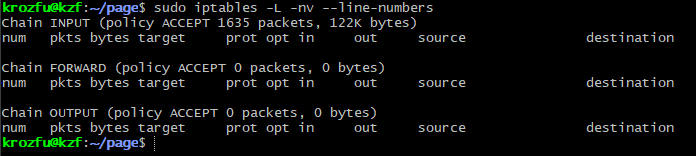
\includegraphics[width=0.75\textwidth]{./assets/img7.png}
  \caption{Estado inicial de las reglas IPTABLES}
  \label{fig:iptables-inicial}
\end{figure}

\subsection{Implementación de Reglas de Filtrado}

\subsubsection{Regla 1: Permitir Tráfico HTTP en Puerto 8080}

Configuramos la primera regla de IPTABLES para aceptar tráfico al puerto HTTP
8080 donde se tiene configurada una página web:

\begin{lstlisting}[
    language=bash, 
    caption=Regla para permitir tráfico HTTP en puerto 8080,
    breaklines=true,
    basicstyle=\small\ttfamily
]
sudo iptables -A INPUT -p tcp --dport 8080 -j ACCEPT
\end{lstlisting}

\textbf{Explicación de la regla:}
\begin{itemize}
  \item \texttt{-A INPUT}: Añade la regla a la cadena INPUT
  \item \texttt{-p tcp}: Especifica el protocolo TCP
  \item \texttt{--dport 8080}: Define el puerto de destino 8080
  \item \texttt{-j ACCEPT}: Acción a ejecutar (aceptar el paquete)
\end{itemize}

\begin{figure}[H]
  \centering
  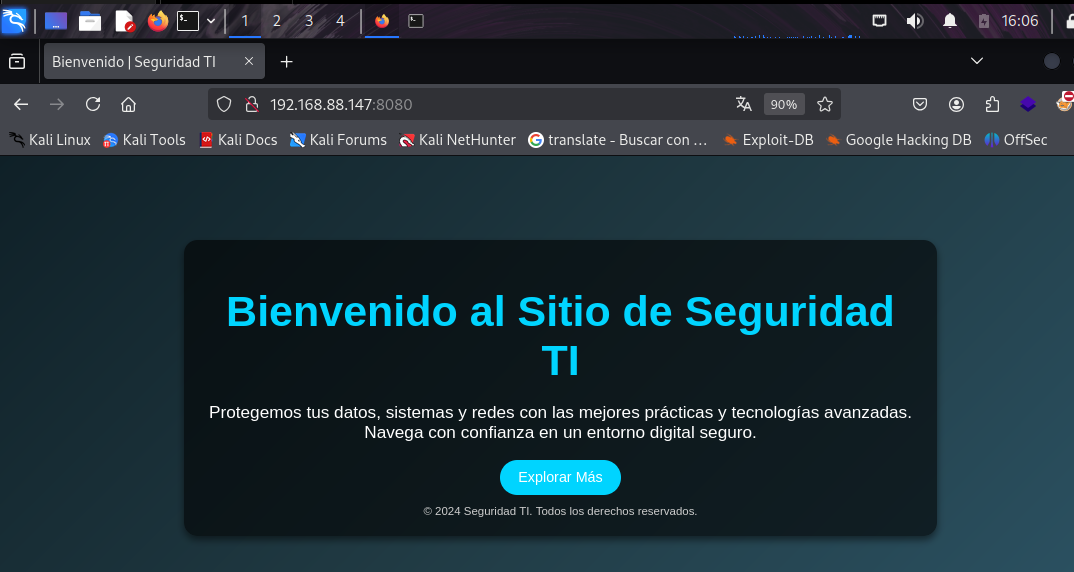
\includegraphics[width=0.75\textwidth]{./assets/img8.png}
  \caption{Regla IPTABLES aplicada para puerto HTTP 8080}
  \label{fig:http-rule}
\end{figure}

\subsubsection{Regla 2: Restricción de Acceso SSH por IP}

Se configura una regla de IPTABLES para permitir el acceso SSH únicamente desde
una dirección IP específica y denegar el acceso desde otros equipos:

\begin{lstlisting}[
    language=bash, 
    caption=Reglas para restricción de acceso SSH,
    breaklines=true,
    basicstyle=\small\ttfamily
]
sudo iptables -A INPUT -p tcp --dport 22 -s 192.168.1.104 -j ACCEPT
sudo iptables -A INPUT -p tcp --dport 22 -j DROP
\end{lstlisting}

\textbf{Explicación de las reglas:}
\begin{itemize}
  \item \textbf{Primera regla}: Permite SSH desde la IP 192.168.1.104
  \item \textbf{Segunda regla}: Deniega SSH desde cualquier otra IP
  \item \texttt{-s 192.168.1.104}: Especifica la IP de origen autorizada
  \item \texttt{-j DROP}: Descarta silenciosamente los paquetes
\end{itemize}

\textbf{Conexión exitosa desde host autorizado:}

\begin{figure}[H]
  \centering
  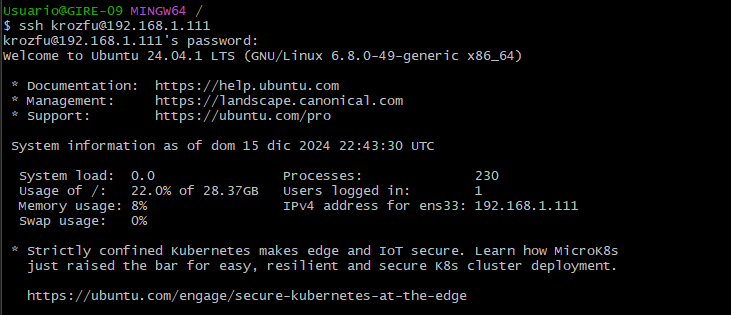
\includegraphics[width=0.75\textwidth]{./assets/img9.png}
  \caption{Conexión SSH exitosa desde IP autorizada (192.168.1.104)}
  \label{fig:ssh-success}
\end{figure}

\textbf{Denegación de conexión desde host no autorizado:}

\begin{figure}[H]
  \centering
  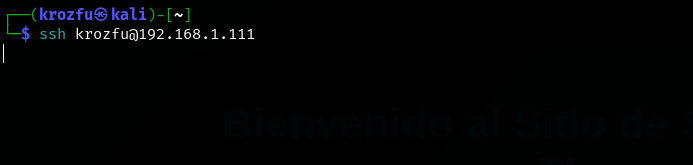
\includegraphics[width=0.75\textwidth]{./assets/img10.png}
  \caption{Conexión SSH denegada desde IP no autorizada}
  \label{fig:ssh-denied}
\end{figure}

\subsubsection{Regla 3: Bloqueo del Servicio DNS}

Se agrega una regla para denegar todo el tráfico relacionado con el servicio
DNS que opera en el puerto 53:

\begin{lstlisting}[
    language=bash, 
    caption=Regla para bloquear tráfico DNS,
    breaklines=true,
    basicstyle=\small\ttfamily
]
sudo iptables -A INPUT -p udp --dport 53 -j DROP
\end{lstlisting}

\textbf{Explicación de la regla:}
\begin{itemize}
  \item \texttt{-p udp}: Especifica el protocolo UDP (usado principalmente por DNS)
  \item \texttt{--dport 53}: Puerto estándar del servicio DNS
  \item \texttt{-j DROP}: Descarta los paquetes DNS entrantes
\end{itemize}

\subsection{Persistencia de Configuración}

\subsubsection{Instalación y Configuración de Persistencia}

Para garantizar que las reglas de IPTABLES permanezcan activas después de un
reinicio del sistema, se ejecutan los siguientes comandos:

\begin{lstlisting}[
    language=bash, 
    caption=Comandos para persistencia de reglas IPTABLES,
    breaklines=true,
    basicstyle=\small\ttfamily
]
sudo apt install iptables-persistent
sudo netfilter-persistent save
sudo netfilter-persistent reload
\end{lstlisting}

\textbf{Función de cada comando:}
\begin{itemize}
  \item \texttt{iptables-persistent}: Instala el paquete para persistencia automática
  \item \texttt{netfilter-persistent save}: Guarda las reglas actuales
  \item \texttt{netfilter-persistent reload}: Recarga las reglas guardadas
\end{itemize}

\subsection{Verificación Final de la Configuración}

Al finalizar el proceso, se puede observar la configuración completa de las
reglas IPTABLES implementadas:

\begin{figure}[H]
  \centering
  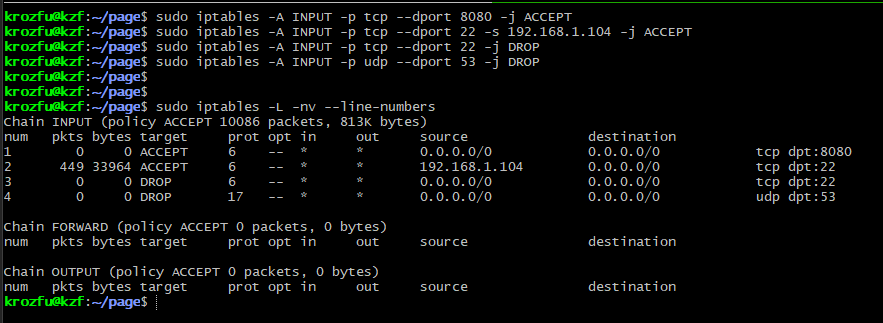
\includegraphics[width=0.75\textwidth]{./assets/img11.png}
  \caption{Configuración final de reglas IPTABLES implementadas}
  \label{fig:iptables-final}
\end{figure}

\textbf{Resumen de reglas implementadas:}

\begin{enumerate}
  \item \textbf{HTTP}: Acceso permitido en puerto 8080
  \item \textbf{SSH}: Acceso restringido solo desde IP 192.168.1.104
  \item \textbf{DNS}: Tráfico UDP bloqueado en puerto 53
  \item \textbf{Persistencia}: Configuración guardada para supervivir reinicios
\end{enumerate}

Esta configuración demuestra un control granular del tráfico de red,
implementando políticas de seguridad específicas para diferentes servicios del
sistema.

% ----------------------------------------------------------------
\section{Despliegue de un IDS con SNORT}

\subsection{Instalación y Configuración Inicial}

\subsubsection{Instalación de Snort en Ubuntu Server}

Se realiza la instalación de Snort en un Ubuntu Server 24.04, descargando la
versión Snort 2.9.20 para configurar el IDS y analizar el tráfico de red[1][2].

\begin{figure}[H]
  \centering
  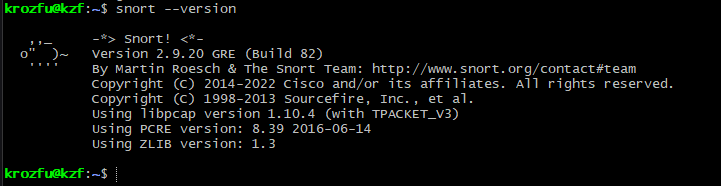
\includegraphics[width=0.75\textwidth]{./assets/img12.png}
  \caption{Instalación de Snort 2.9.20 en Ubuntu Server 24.04}
  \label{fig:snort-installation}
\end{figure}

\subsubsection{Configuración del Modo Promiscuo}

Se habilita el modo promiscuo en la interfaz de red para permitir que Snort
capture todo el tráfico que pasa por la red, no solo los paquetes dirigidos
específicamente al host:

\begin{lstlisting}[
    language=bash, 
    caption=Habilitación del modo promiscuo en la interfaz de red,
    breaklines=true,
    basicstyle=\small\ttfamily
]
sudo ip link set ens33 promisc on
\end{lstlisting}

\textbf{Función del modo promiscuo:}
\begin{itemize}
  \item Permite capturar todo el tráfico de red que pasa por el segmento
  \item Esencial para el funcionamiento efectivo de un IDS de red
  \item Habilita la detección de ataques dirigidos a otros hosts de la red
\end{itemize}

\subsection{Configuración del Archivo Principal}

\subsubsection{Modificación de snort.conf}

Se procede a modificar las reglas en el archivo \texttt{snort.conf} para
configurar las variables necesarias que permitan a Snort detectar posibles
intrusiones[3]:

\begin{figure}[H]
  \centering
  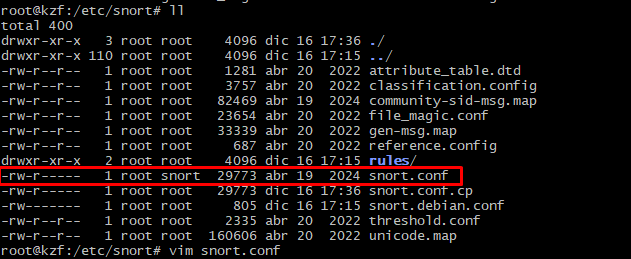
\includegraphics[width=0.75\textwidth]{./assets/img13.png}
  \caption{Configuración de variables en el archivo snort.conf}
  \label{fig:snort-conf}
\end{figure}

Se modifican las siguientes variables principales para optimizar la captura de
tráfico:

\begin{itemize}
  \item \textbf{\$HOME\_NET}: Define la red local a proteger
  \item \textbf{\$EXTERNAL\_NET}: Especifica las redes externas (generalmente \texttt{!HOME\_NET})
  \item \textbf{\$RULE\_PATH}: Directorio donde se almacenan las reglas de detección
  \item Variables de puertos para servicios específicos (HTTP, SSH, DNS, etc.)
\end{itemize}

\subsubsection{Configuración de Reglas Personalizadas}

Se modifica el archivo \texttt{local.rules} donde se configuran las reglas
personalizadas que tendrá Snort para el análisis de tráfico:

\begin{figure}[H]
  \centering
  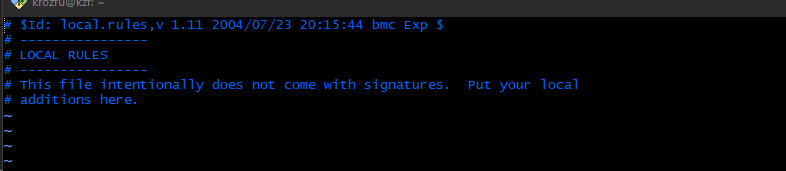
\includegraphics[width=0.75\textwidth]{./assets/img14.png}
  \caption{Archivo local.rules para reglas personalizadas de Snort}
  \label{fig:local-rules}
\end{figure}

\subsection{Implementación de Reglas de Detección}

\subsubsection{Regla de Detección ICMP}

Se implementa una regla personalizada para detectar tráfico ICMP dirigido hacia
la red local. La estructura de las reglas Snort sigue el formato estándar con
cabecera y opciones[2][3]:

\begin{lstlisting}[
    language=text, 
    caption=Regla Snort para detección de tráfico ICMP,
    breaklines=true,
    basicstyle=\small\ttfamily
]
alert icmp any any -> $HOME_NET any (msg:"ICMP ping detectado en el sistema"; sid:1000001)
\end{lstlisting}

\textbf{Estructura de la regla explicada:}
\begin{itemize}
  \item \textbf{alert}: Acción a ejecutar cuando se detecte el patrón
  \item \textbf{icmp}: Protocolo a monitorear
  \item \textbf{any any}: IP y puerto de origen (cualquiera)
  \item \textbf{->}: Dirección del tráfico
  \item \textbf{\$HOME\_NET any}: IP y puerto de destino
  \item \textbf{msg}: Mensaje de alerta personalizado
  \item \textbf{sid}: Identificador único de la regla (debe ser > 1000000 para reglas locales)
\end{itemize}

\begin{figure}[H]
  \centering
  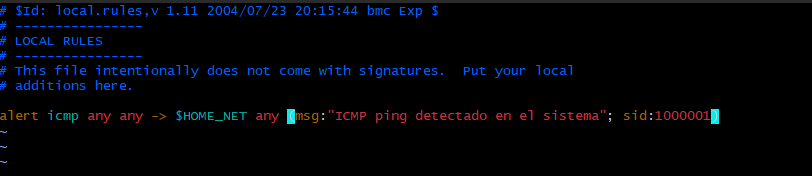
\includegraphics[width=0.75\textwidth]{./assets/img15.png}
  \caption{Implementación de la regla ICMP en local.rules}
  \label{fig:icmp-rule}
\end{figure}

\subsection{Validación y Pruebas del Sistema}

\subsubsection{Verificación de Configuración}

Se ejecuta la validación de la configuración de Snort para asegurar que todas
las reglas estén correctamente implementadas:

\begin{lstlisting}[
    language=bash, 
    caption=Comando de validación de configuración Snort,
    breaklines=true,
    basicstyle=\small\ttfamily
]
snort -T -c /etc/snort/snort.conf
\end{lstlisting}

\begin{figure}[H]
  \centering
  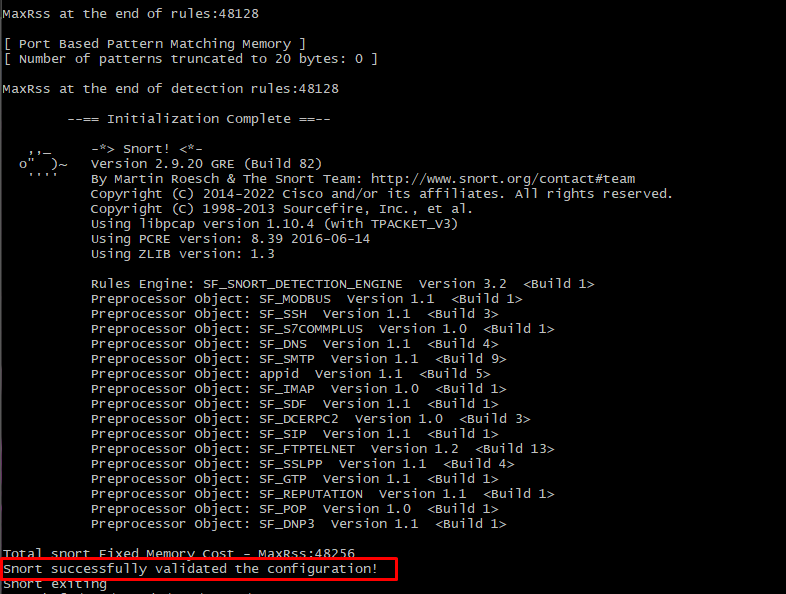
\includegraphics[width=0.75\textwidth]{./assets/img16.png}
  \caption{Resultado exitoso de la validación de configuración}
  \label{fig:config-validation}
\end{figure}

\subsubsection{Ejecución del IDS en Modo Detección}

Se inicia Snort en modo de detección activa para monitorear el tráfico de red
en tiempo real:

\begin{lstlisting}[
    language=bash, 
    caption=Comando para ejecutar Snort en modo IDS,
    breaklines=true,
    basicstyle=\small\ttfamily
]
sudo snort -q -l /var/log/snort -i ens33 -A console -c /etc/snort/snort.conf
\end{lstlisting}

\textbf{Parámetros del comando:}
\begin{itemize}
  \item \textbf{-q}: Modo silencioso (quiet mode)
  \item \textbf{-l /var/log/snort}: Directorio para almacenar logs
  \item \textbf{-i ens33}: Interfaz de red a monitorear
  \item \textbf{-A console}: Mostrar alertas en consola
  \item \textbf{-c}: Archivo de configuración a utilizar
\end{itemize}

\subsection{Pruebas de Detección}

\subsubsection{Generación de Tráfico de Prueba}

Desde una máquina con Kali Linux se ejecuta un envío de trazas ICMP para
verificar el funcionamiento de la regla de detección implementada:

\begin{figure}[H]
  \centering
  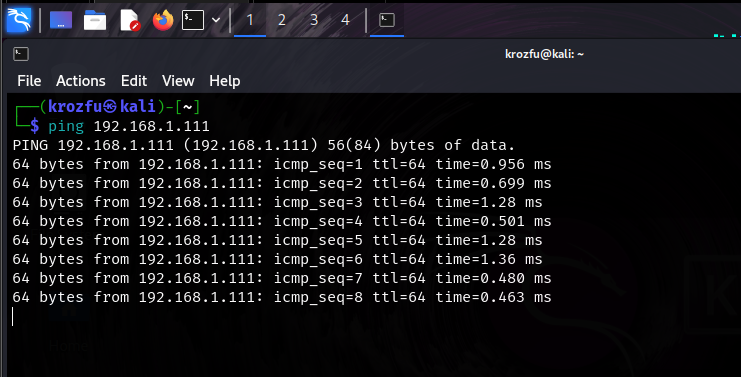
\includegraphics[width=0.75\textwidth]{./assets/img17.png}
  \caption{Generación de tráfico ICMP desde Kali Linux}
  \label{fig:icmp-traffic}
\end{figure}

\subsubsection{Detección y Alertas}

Snort detecta exitosamente el tráfico ICMP generado, mostrando las alertas
correspondientes con la información de origen y destino:

\begin{figure}[H]
  \centering
  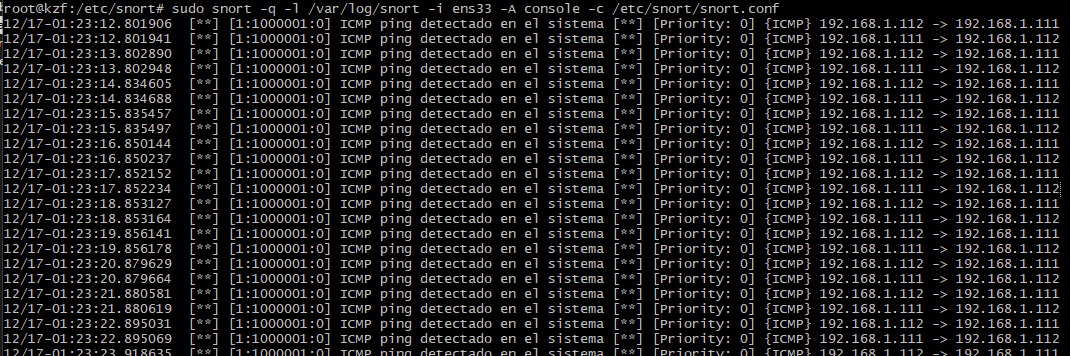
\includegraphics[width=0.75\textwidth]{./assets/imga18.png}
  \caption{Alertas de Snort detectando tráfico ICMP}
  \label{fig:snort-alerts}
\end{figure}

\textbf{Información capturada en las alertas:}
\begin{itemize}
  \item Timestamp de la detección
  \item Dirección IP de origen y destino
  \item Protocolo utilizado (ICMP)
  \item Mensaje personalizado de la regla
  \item Identificador de la regla activada (SID)
\end{itemize}

\subsection{Resultados de la Implementación}

La implementación del IDS con Snort ha demostrado ser exitosa, logrando:

\begin{enumerate}
  \item \textbf{Instalación correcta} de Snort 2.9.20 en Ubuntu Server 24.04
  \item \textbf{Configuración adecuada} del modo promiscuo para captura de tráfico
  \item \textbf{Implementación exitosa} de reglas personalizadas de detección
  \item \textbf{Detección efectiva} de tráfico ICMP según las reglas configuradas
  \item \textbf{Generación de alertas} en tiempo real con información detallada
\end{enumerate}

Este sistema IDS proporciona una base sólida para la detección de intrusiones y
puede expandirse con reglas adicionales para detectar otros tipos de amenazas
de seguridad.

% ----------------------------------------------------------------
\section{Conclusiones}

\begin{itemize}
  \item Se logró implementar un ecosistema de seguridad integral que abarca desde la
        prevención de ataques de inyección SQL hasta la detección de intrusiones,
        demostrando la importancia de un enfoque de defensa en profundidad. La
        combinación de módulos de filtrado, servidores seguros con TLS/SSL, firewalls
        con IPTABLES y sistemas de detección con Snort proporciona una protección
        robusta contra diversas amenazas.
  \item El módulo desarrollado para prevenir ataques de SQL Injection demostró ser
        altamente efectivo, bloqueando exitosamente intentos de ataques como UNION
        SELECT y bypass de autenticación mediante el uso de prepared statements y
        validación de entrada. La comparación entre el sistema vulnerable y el
        protegido evidenció claramente la importancia de implementar estas
        contramedidas en aplicaciones web.
  \item La implementación del servidor HTTPS con certificados SSL/TLS autofirmados y el
        sistema de firma digital con PGP destacaron la relevancia de la criptografía
        para garantizar la confidencialidad, integridad y autenticidad de las
        comunicaciones. Aunque los certificados autofirmados generan advertencias de
        seguridad, proporcionan el cifrado necesario para entornos de desarrollo y
        pruebas.
  \item La configuración de reglas de firewall con IPTABLES permitió implementar
        políticas de seguridad específicas y granulares, demostrando cómo se puede
        controlar efectivamente el acceso a servicios críticos como SSH, HTTP y DNS. La
        capacidad de restringir acceso por IP específica y la persistencia de las
        reglas garantizan un control continuo del tráfico de red.
  \item El despliegue de Snort como sistema de detección de intrusiones proporcionó
        capacidades de monitoreo en tiempo real, demostrando su efectividad para
        detectar patrones de tráfico sospechoso como paquetes ICMP. La configuración
        del modo promiscuo y las reglas personalizadas permiten una detección proactiva
        de amenazas, complementando las medidas preventivas implementadas en las otras
        capas de seguridad.

\end{itemize}

\end{document}
